\chapter{Typing Dependency Structure}
\label{chapter:chapter_2}

\chapabstract{
	Predicates are functors,\\
	complements -- diamonds,\\
	adjuncts -- boxes;\\
	Everything a type.
}

The previous chapter initiated us into the history-rich world of substructural logics in the intuitionistic tradition.
Along the (artificially homogenized) story, we got to dip our toes into linguistic waters, where we saw these logics thrive and prosper, finding their place as the foundation for categorial grammars.
The many flavours of categorial grammars all have a single common denominator: they treat syntax as a hierarchical structure that puts phrases together from small to big, starting from words and reaching up to the sentence, the imprint being a natural deduction tree (and perhaps a phrasal bracketing structure).
This emphasis on the phrase, combined with the distinctive shape of the categorial parse, allows for a partial parallel to be drawn between categorial grammars and phrase structure grammars, despite their stark methodological and theoretical contrasts.
Phrase structure grammars are rule-based systems that assign categories to phrases according to their syntactic function, and manipulate phrasal formation by specifying how their constituent parts combine -- the produce being a bracketing structure, commonly visualized in tree format.
A different approach to grammatical theory abandons the constituency relation, adopting the dependency relation in its stead.
Dependency relations do not seem compatible with the categorial setup at a first glance: they are flat, and lack the notion of finite phrasal parts -- in showing no attachment to iterative phrasal division, they are also not obviously compositional.

In this, chapter we will focus our efforts into bridging this gap between these two perspectives under a unified categorial grammar setup.
We will motivate the incorporation of dependency relations into the categorial vocabulary by repurposing existing and well-studied tools that remain faithful to the type theory roots the previous chapter has established (hint: it's the modalities).
We will finally discuss how their inclusion alters the structural paradigms of the previous chapter, and the opportunities and problems this change comes with.

\section{Phrase vs. Dependency Structure}
\label{section:phrase_vs_dependecy}
Before we get to theorycrafting, it would be useful to try and clarify what exactly is meant by constituency- and dependency- structure, and how the two differ.

\subsection{Phrase Structure Grammars}
Phrase structure grammars build on the observation that certain phrases seem to act as rigid and independent chunks, sometimes referred to as \textit{constituents}. 
Viewed from within, these phrases may be rich in internal structure, but keep it sealed off to the outside.
Viewed externally (i.e. in the context of a wider phrase that contains them), they are indivisible units, or at least for the purposes of phrasal composition.
Phrases are inventorized according to their syntactic \textit{categories}.
If one so wishes, they can for the most part replace a phrase for another of the same category, with no effect to grammaticality or local structure, which suggests they are functionally indiscernible.
The examples below testify to this%
\footnote{Sourced from H.P. Lovecraft, \textit{Celepha\"{i}s}  (1922). In \textit{The Rainbow, vol. 2.}}; the underlined phrases can be freely interchanged -- despite their wildly different internal structures, substituting one for another has no effect on the outer sentential structure:

{\smaller%
\begin{enumerate}
\item $\w{he}\sbind(\w{beheld}\sbind\underline{(\w{the}\sbind\w{city})})$
\item $\w{he}\sbind(\w{beheld}\sbind\underline{(\w{the}\sbind((\w{glittering}\sbind{\w{minarets}})\sbind(\w{of}\sbind(\w{the}\sbind\w{city}))))})$
\item $\w{he}\sbind(\w{beheld}\sbind(\underline{(\w{such}\sbind\w{beauty})\sbind(\w{of}\sbind((\w{red}\sbind(\w{and}\sbind\w{white}))\sbind\w{flowers})))})$
\item $\w{he}\sbind(\w{beheld}\sbind(\underline{
	(
		\w{some}\sbind
			(\w{feature}\sbind
				(\w{or}\sbind\w{arrangement})
			)\!\sbind\!
			(\w{which}\sbind
				(\w{he}\sbind
					(
						(\w{had}\sbind\w{known})\sbind
						\w{before}
					)					
				)
			)})$
\end{enumerate}}%

\noindent These so-called constituents interact, then, with one another depending not on their contents, but rather their categories.
This perspective promotes a disciplined approach to grammar modeling, dating back to the formal grammars of \citet{chomsky1956three}, the archetypical example being context-free grammars~\cite{chomsky1956three,jw1959c}.
There, the construction of complex expressions is guided by \textit{production rules}, grammatical recipes that dictate what categories can sequentially combine, in what order, and what the category of their combination is.
The above example would correspond, for instance, to production rules of the form:
\begin{align}
	S 	& 	\to NP \ VP \label{equation:sfromnpvp}\\
	VP 	&	\to TV \ NP \label{equation:vpfromtvnvp}
\end{align}
claiming that one of the ways to make a verb phrase $VP$ involves concatenating a transitive verb $TV$ with a noun phrase $NP$, which in turn can be plugged to the right of another $NP$ to produce a declarative sentence $S$ -- each rule leaving a bracketing structure (or binary tree) in its wake (see Figure~\ref{subfigure:cfgtree}).


\begin{figure}
	\centering
	\hfill%
	\begin{subfigure}[b]{0.35\textwidth}
		\begin{tikzpicture}
			\Tree 
				[ .{$S$} 
					[.{(\ref{equation:sfromnpvp})}
						[.{$NP$} 
							\w{he} 
						] 
						[.{$VP$}
							[.{(\ref{equation:vpfromtvnvp})} 
								[.{$TV$} \w{beheld} ] 
								[.{$NP$} 
									\edge[roof]; {\dots} 
								] 
							]
						] 
					]
				] 
		\end{tikzpicture}
		\caption{Context-free parse tree.}
		\label{subfigure:cfgtree}
	\end{subfigure}\hfill%
	\begin{subfigure}[b]{0.45\textwidth}
		\begin{tikzpicture}
			\Tree 
				[ .\s[s]
					[.{$\appleft$}
						[.{\np[s]}
							\w{he}
						]
						[.{$\np[s]\divleft\s[s]$}
							[.{$\appright$}
								[.{$(\np[s]\divleft\s[s])\divright\np[s]$} \w{beheld} ]
								[.{\np[s]}
									\edge[roof]; {\dots}
								]
							]
						]
					]
				]
		\end{tikzpicture}
		\caption{Tree-formatted Lambek derivation.}
		\label{subfigure:lambektree}
	\end{subfigure}\hfill
	\caption{A phrase-structure grammar parse tree (\subref{subfigure:cfgtree}) contrasted with a Lambek abstract syntax tree (\subref{subfigure:lambektree}).}
	\label{figure:cfgvslambek}
\end{figure}

Even though context-free grammars are no longer seriously considered in the linguistic world, they have directly influenced most early attempts at grammar design -- and, by extension, their later successors and refinements.
Notational evidence of this past are more than noticeable today, ranging from the wide adoption of tree-style notation for syntactic analyses to the conceptual syncretism of constituency grammars and phrase structure ones.
More up-to-date frameworks expand upon the barebones context-free backend with niceties like a separation of functional dominance and linear precedence, added rules that manipulate movement and discontuinity, the proclamation of a single category as the \textit{head} of a production rule (or subtree), feature markings that carry semantic, morphological or phonological information, incorporation of dependency information, etc.~\cite[inter alia]{gazdar1985generalized,jacobson1987phrase,pollard1994head,dalrymple2001lexical}.

To our ill fortune, the field of formal syntax is actually an informal mess, more akin to a mine field rather than an academic one; it's best if I tread carefully and refrain from overextending myself here, in order to avoid setting off unseen traps or causing easily avoidable confusion.
The point I want to make is that the focal center of the above formalisms is the \textit{phrase} and its structure -- as such, they are all referred to as phrase structure grammars, regardless of whatever extra fluff they carry or what their expressive capacity is.
In that broader sense of the term, and removing any implicit connotations of intellectual lineage, categorial grammars can also be conceived as phrase-centric.
Pure Lambek systems, for one, also explicate how phrases are combined, adhere to hierarchical forms similar to those of context-free grammars (except beautifully, see Figure~\ref{subfigure:lambektree}) and in fact have the same expressive capacity with respect to string formation (i.e. the two are \textit{weakly} equivalent)~\cite{pentus1993lambek}.
Categorial grammars abstract away from the rule inventory by utilizing the smallest and purest set of rules possible -- those of function application and variable abstraction -- and internalize what used to be rule-imposed structure within the lexical categories themselves.
Bracketing structure is now the footprint of function application, and the interface with semantics is naturalized by virtue of the Curry-Howard correspondence, as we saw earlier.
Rather than a $VP$ category and rule~(\ref{equation:sfromnpvp}), we have the \textit{type} $\np[s]\divleft\s[s]$ -- transparent with respect to both its syntactic combinatorics and semantic function.
Performing the function application on a left-adjacent \np[s] will then result to a local tree structure, not unlike the corresponding production rule -- see Figure~\ref{figure:cfgvslambek} for a comparison.
Note that in reality, categorial derivations in the type-theoretic tradition resemble trees only locally, since in high-order phenomena involving abstractions the unary, non-terminal $\lambda$ nodes will either need to be uniquely named with the variable they are binding, or otherwise point to it  with an additional edge -- hence a directed acyclic graph could make for a more accurate representation format.
Long story short, even without extensions to the logical core for managing discontuinity, calling deductive parsing constituency parsing would obviously not be doing the former justice; yet despite their methodological and theoretical divergences, their end yield is comparable -- the antecedent structures of Figures~\ref{figure:nl_applicative_examples} to~\ref{figure:lovecraft_coord} testify that the former may in fact be seen as subsuming the latter.

\subsection{Dependency Grammars}
\label{subsection:dep_grammars}
The constituency tradition has co-evolved along the opposing view of dependency grammars~\cite[inter alia]{tesniere2015elements,gaifman1965dependency,sgall1986meaning,mel1988dependency,sleator1995parsing}.
Dependency grammars reject the binary phrasal division that constituency grammars abide by, and instead adopt a flatter structural form, the only unit of which is the word.
Words are connected with one another by dependency arcs, i.e. directed edges between word pairs.
Each word can have arbitrarily many outgoing edges (dependents), but only a single incoming edge (head) -- the exception is the root word which has no head of its own (i.e. the head of the matrix clause).
A word is said to directy dominate its dependents, and indirectly dominate all words its dependents dominate (directly or otherwise) -- e.g. the root indirectly dominates every other word in the sentence.
This distinction between head and dependent is central to dependency grammars; broadly speaking, heads can be thought of as the words that decide the syntactic functionality of the collection of words (for fear of calling it a phrase) they indirectly dominate.
The dependency structure of a sentence is once more a tree, with words now as both terminal and non-terminal nodes, glued together with dependency relations.
A dependency tree is unconstrained by adjacency and word order: edges can fly over other edges; planarity is optionaly respected: an edge penetrating another edge to enter a nested domain is called \textit{non projective}.
This perspective is computationally appealing due to its simplicity and uniformity, as it allows a dependency grammar to argue about languages with wildly diverging syntactic and typological properties while remaining virtually unchanged.
For the exact same reasons, it can also be seen as concealing -- it sacrifices any potential of targeted analysis in the pedestal of universality.
Finally, the semantically inclined might find a two-directional extension of dependency arcs enticing.
In that setup, the added direction (which needs not agree with that of syntactic dominance) is devoted to semantic information flow, pointing from semantic predicates%
	\footnote{Apparently also an overloaded term. I will only ever use this in the strictly logical sense.},
to semantic arguments~\cite{mel2003levels}.

A dependency grammar that has gained significant traction over the last decade is the framework of universal dependencies~\cite{10.1162/coli_a_00402}, claiming a broad collection of multi-lingual treebanks~\cite{nivre2020universal} and tools.
In universal dependencies, words are usually assigned a label pulled from a rudimentary set of part of speech tags and lexical identifiers and more importantly, dependency relations are also labeled according to their grammatical function, allowing the distinction of a words' dependents according to the grammatical role they fulfill.
Grammatical roles are typologically and thematically informed, and are inventorized with language universality as the prime goal.
This inventorization upholds no semantic promises, but is not inconsistent with the aforementioned semantic view either.
To obtain a semantic transcription of the dependency tree, one needs only specify whether the semantic flow of each grammatical role is co- or contra- directional to the edge's syntactic flow, i.e. whether the arc marks its dependent as a \textit{complement} (where syntactic head and semantic predicate coincide) or an \textit{adjunct} (where the syntactic head is the semantic argument to its syntactic dependent).%
	\footnote{Universal dependencies, a staunch pacifist, carefully and vocally refuses to make this claim, as complements and adjuncts are largely language-particular syntactic constructs and a notorious point of debate~\cite{haspelmath2014arguments}.
	I would like to believe I am not trespassing here, either -- as will be made clearer in a bit, I employ the two terms in a purely semantic fashion.}

\begin{figure}
	\centering
	\begin{tikzpicture}[t/.style={text height=1.5ex, text depth=.25ex, rectangle, outer sep=0pt}, node distance=10pt]
	\smaller
	\node[t] (he) 			at (0, 0) {\w{he}};
	\node[t] (he_)			[below=4pt of he] {\w{PRON}};
	\node[t] (beheld)		[right=10pt of he] {\w{beheld}};
	\node[t] (beheld_)		[below=4pt of beheld] {\w{VERB}};
	\node[t] (the) 			[right=10pt of beheld] {\w{the}};
	\node[t] (the_)			[below=4pt of the] {\w{DET}};
	\node[t] (glittering) 	[right=10pt of the] {\w{glittering}};
	\node[t] (glittering_)	[below=4pt of glittering] {\w{VERB}};
	\node[t] (minarets)		[right=10pt of glittering] {\w{minarets}};
	\node[t] (minarets_)	[below=4pt of minarets] {\w{NOUN}};
	\node[t] (of)			[right=10pt of minarets] {\w{of}};
	\node[t] (of_)			[below=4pt of of] {\w{ADP}};
	\node[t] (the2)			[right=10pt of of] {\w{the}};
	\node[t] (the2_)		[below=4pt of the2] {\w{DET}};
	\node[t] (city)			[right=10pt of the2] {\w{city}};
	\node[t] (city_)		[below=4pt of city] {\w{NOUN}};
	\draw[->] (beheld) [bend right=80] edge node [above] {\smaller[2]{nsubj}} (he);
	\draw[->] (beheld) [bend left=90] edge node [above] {\smaller[2]{dobj}} (minarets);
	\draw[->] (minarets) [bend right=40] edge node [above] {\smaller[2]{amod}} (glittering);
	\draw[->] (minarets) [bend right=70] edge node [above] {\smaller[2]{det}} (the);
	\draw[->] (minarets) [bend left=60] edge node [above] {\smaller[2]{prep}} (of);	
	\draw[->] (of) [bend left=90] edge node [above] {\smaller[2]{pobj}} (city);	
	\draw[->] (city) [bend right=60] edge node [above] {\smaller[2]{det}} (the2);
	\end{tikzpicture}
	\caption{A sample dependency parse in the universal dependencies format.}
	\label{figure:udparse}
\end{figure}

Figure~\ref{figure:udparse} shows an example dependency parse.
Unlike before, we can not claim any semblance to the proofs that have occupied us thus far.
At a first glance, dependency grammars have little in common with categorial grammars -- structures are no longer binary nor made out of phrases, the axis of grammatical functions is competely new, and there seems to be little there reminiscent of the notions of induction and composition.
Though on closer inspection and armed with some goodwill, we can recover from some of these divergences if we make a few concessions from both sides.
We can start by treating any collection of words rooted in the same ancestor in the dependency tree as a constituent phrase, albeit possibly discontinuous -- the result will give us at least some partial overlap with the categorial directive.
Grammatical functions can then be thought of as being implicit, having been internalized in their positioning within a functor.
For instance we do intuitively know that the Lambek transitive verb $(\np[s]\divleft\s[s])\divright\np[s]$ requires an \textit{object} $\np[s]$ to the right and a \textit{subject} $\np[s]$ to the left -- marking them as such is perhaps redundant, since the verbal meaning recipe places each syntactic argument into a distinct semantic slot.
The binary bracketing structure is irrevocably lost, but this loss can be deemed as inconsequential if we ``flatten'' functor-induced phrasal boundaries by considering them only at these intermediary points where all of their arguments (however many) have been applied.
It is not much further we can get with this mediatory role, though.
No concession from the categorial side would be able to justify the underspecification of higher-order phenomena in a dependency tree,
and no concession from the dependency side could make peace with the omission of the concept of headedness in an applicative natural deduction proof.

\section{Modalities for Dependency Demarcation}
\label{section:modalities_for_dependency}
In our new quest, we will seek to design a type logic that subsumes and rises above both phrase structure grammars and dependency grammars.
As we saw in the previous section, the bar is not set particularly high for the first kind; the Lambek calculus can already do more than well enough.
The challenge then is to integrate the added values of a dependency grammar in a type-theoretic framework.
There's two elements we are missing; distinguishing between syntactic heads and syntactic/semantic predicates, and marking words and phrases according to their grammatical roles within some wider context.

\subsection{Two Dimensional Predicates}
Categorial grammars are inherently and by design biased towards predicate structures, primarily syntactic, but simultaneously also semantic (if one is to believe the story of Section~\ref{subsubsection:ssi_tlg}, no distinction can be made between the two).
Each phrase can be iteratively split apart into two subphrases (not necessarily contiguous), where one provides a functor, and the other the argument thereof.
Note that this distinction does not preclude the possibility that the argument itself has a functional type -- no assumption is made on the form of either subphrase's type, other than the two being compatible.
But what assumes the role of the functor in a local domain needs not always be the syntactic head of that domain.
There's a plethora of example cases.
Quantifiers, for one, are inarguably predicates over the objects they quantify, yet they exactly obey the morphosyntactic characteristics prescribed by these objects (i.e. grammatical gender, case, number, etc.), evidencing that the latter are in fact the heads -- a clear violation of any alignment between syntactic predicate and syntactic head we could ever hypothesize. 
A similar argument can be made for determiners and, more broadly speaking, any phrasal element that takes functional precedence without being the syntactically prominent part of its phrase, e.g. adjectival and adverbial modifiers.

This observation gives rise to a binary subcategorization of a binary predicate structure; to establish some risky terminology, it is either:
\begin{enumerate}
	\item an application of a head to its \textit{complement}, or
	\item an application of an \textit{adjunct} to its head
\end{enumerate}
where the distinction between complement and adjunct is made solely on the basis of their functional relation to the head.

The vanilla categorial vocabulary does not suffice to capture this extra dimension of function application -- a problem also noticed by the intellectuals of proto-categorial civilizations, as archeological excavations reveal.
In an unpublished manuscript, \citet{moortgat1991heads} propose a two-dimensional implicational type operator and corresponding residuation laws: the first binary dimension is reserved for the usual left- vs. right- application distinction, whereas the second binary dimension specifies whether the head occurs to the left or to the right; the result is four unique ways of building up an implication.
Congruent with the substructural trend of revealing structure that was once hidden, this division brings forth a two-valued structural binder, allowing the corresponding logic $\logic{DNL}$ to reason about \textit{headed} binary trees.
The authors refrain from commiting to a specific linguistic application, but, translated into our terminology, their proposal can be schematically summarized by Figure~\ref{figure:heads_and_phrases}.
Further away from syntax, \citet{hendriks1997logic} employs \logic{DNL} to account for prosodic structures, where the head is assigned to intonationally prominent elements.

\begin{figure}
	\centering
	\begin{tabularx}{0.7\textwidth}{@{}lXr@{}}
	\begin{tikzpicture}[level distance=60pt, sibling distance=30pt,
						t/.style={text height=1.5ex, text depth=.25ex, rectangle, outer sep=0pt}, node distance=10pt]
	\Tree [.{$\prop{b}$} \edge[head] node[midway,left,t]{$\textit{head}$}; {$\prop{b}\divright_l\prop{a}$} \edge node[midway,right,t]{$\textit{complement}$}; {$\prop{a}$} ]
	\end{tikzpicture}
	&
	&
	\begin{tikzpicture}[level distance=60pt, sibling distance=30pt,
						t/.style={text height=1.5ex, text depth=.25ex, rectangle, outer sep=0pt}, node distance=10pt]
	\Tree [.{$\prop{b}$} \edge node[midway,left,t]{$\textit{complement}$}; {$\prop{a}$} \edge[head] node[midway,right,t]{$\textit{head}$}; {$\prop{a}\divleft_r\prop{b}$} ]
	\end{tikzpicture}\\[\smallsep]
	\begin{tikzpicture}[level distance=60pt, sibling distance=30pt,
						t/.style={text height=1.5ex, text depth=.25ex, rectangle, outer sep=0pt}, node distance=10pt]
	\Tree [.{$\prop{b}$} \edge[head] node[midway,left,t]{$\textit{head}$}; {$\prop{a}$} \edge node[midway,right,t]{$\textit{adjunct}$}; {$\prop{a}\divleft_l\prop{b}$} ]
	\end{tikzpicture}
	&
	&
	\begin{tikzpicture}[level distance=60pt, sibling distance=30pt,
						t/.style={text height=1.5ex, text depth=.25ex, rectangle, outer sep=0pt}, node distance=10pt]
	\Tree [.{$\prop{b}$} \edge node[midway,left,t]{$\textit{adjunct}$}; {$\prop{b}\divright_r\prop{a}$} \edge[head] node[midway,right,t]{$\textit{head}$}; {$\prop{a}$} ]
	\end{tikzpicture}\\
	\end{tabularx}
	\caption{The four implications of \logic{DNL}.}
	\label{figure:heads_and_phrases}
\end{figure}

\subsection{Modal Dependents}
As an alternative to introducing implicational (and by residuation, product) variants, we can instead opt for the more fashionable modal decomposition approach~\cite{kurtonina1997structural}.
The allows us to view a specialized (here: head-aware) implicational variant as a composition of its uniform base with a unary modality.
The standard route would have use the modality to mark the head -- we will instead mark the dependent.
More than a petty act of rejection to establishment, this shall provide us with the means to further differentiate dependents according to the exact grammatical slots they occupy -- after all, there's quite a few different dependency labels, but only the one head.

\subsubsection{Complements vs. Adjuncts}
Sticking to our risky agenda, the first distinction we need to make is that of complements versus adjuncts.
In the complement case, such a decomposition would look as follows:
\begin{align}
	\prop{b} \divright_l \prop{a} \ \equiv \ \prop{b} \divright \diamond \prop{a} \\
	\prop{a} \divleft_r \prop{b} \ \equiv \ \diamond  \prop{a} \divleft \prop{b}
\end{align}
The translation is straightforward: predicates in head position are functors requiring the same arguments as they would before, except now under a diamond.
In that sense, they \textit{assign} diamonds to their complements by necessitating an application of the $\diamond I$ rule of Figure~\ref{figure:modal_logical} prior to the function application.
Recalling the structural imprint of the rule, this results in an extra layer of bracketing structure the delimits complement phrases and isolates them from their surroundings.

The adjunct case may at first glance seem slightly more obscure.
Following the directives of the previous paragraph, we need to mark the dependent -- this time a predicate in non head position -- in a way such that its application on its argument leaves a bracketing imprint on the structure of the former rather than the latter.
The solution manifests in the form of a box:
\begin{align}
	\prop{b} \divright_r \prop{a} \ \equiv \ \bx (\prop{b} \divright \prop{a}) \\
	\prop{a} \divleft_l \prop{b} \ \equiv \ \bx (\prop{a} \divleft \prop{b})
\end{align}
The translation is not much different: adjuncts are predicates wrapped by a box.
To reveal the pure function contained therein and allow a proof to progress, we need to invoke the $\bx E$ rule of Figure~\ref{figure:modal_logical}, the effect being a bracketing structure that now delimits adjunct phrases.

There is symmetry between the above two cases.
The task of imposing dependency structure is always upon the functional predicate and its type.
Head predicates mark their complements, whereas adjunct predicates mark themselves; in either case, it is the dependent structure that gets the brackets.
The duality of predicate structure is thus mirrored in the innate distinction between function and argument of the applicative categorial backend, whereas the duality of syntactic headedness is captured by the unary modalities; type-checking in both dimensions.

\subsubsection{Grammatical Functions}
Let's take this a bit further.
Universal dependencies may make no adjunct vs. complement distinction, but they go the extra mile of subspecifying dependents according to the exact grammatical roles they play.
Extending our grammar logic accordingly is trivial.
Rather than have a single diamond and box, we can consider a usecase where modalities are a \textit{family} of unary residuals, i.e. a set of pairs, each labeled according to a single, unique dependency label.
The generalization is a multimodal type system consisting of modal pairs:
\begin{equation}
\{(\ddia{d}, \dbox{d}) \ | \ {\dep{d} \in \deps} \} 
\end{equation}
where \deps{} the full set of dependency labels made available to each specific instantiation of the theory.%
\footnote{Note that the label set can vary depending on the designer's end goal; grammatical functions is just one of the possibilities.
	The setup is also more than compatible with frame semantics, where event-specific semantic structures (\textit{frames}) are evoked by lexicalized syntactic heads to assign semantic/thematic roles to their dependents (\textit{frame elements})~\cite{fillmore1976frame}.}%
The edge case of \deps{} being a singleton set collapses to the previous exposition (whereby explicit labeling is redundant).

Each instance of a labeled modality will now come with its own introduction and elimination rules.
Concomitantly, both the term calculus and the bracketing structures are extended with multiple labels; the modal rewrites and unary brackets of Section~\ref{subsec:modal_logic} are now differentiated on the basis of the dependency label that induced them.
Unlike before, the structural effect is not a means to the end of structural reasoning, but the very purpose of the dependency modalities -- as such, they are not necessarily associated with any structural rules (even though nothing precludes the possibility -- it might even be reasonable to condition each dependency or combinations thereof to a unique set of structural irregularities, as we will see in a bit).
Note, also, that the residuation properties and normalization routines apply only between diamonds and boxes of the \textit{same label} -- no interaction between mismatched types and terms is stipulated.


\subsection{Inference with Dependency-Enhanced Types}
Logical inference in the setup envisaged here is not dissimilar conceptually to the standard type-logical pipeline of Section~\ref{subsection:typelogical}, but there's some crucial differences that require explication, plus a few critical gotchas to beware of.

\subsubsection{Initial Lexical Adjustments}
For starters, functors previously involved with simple applicative phenomena will now need to abide to either of the type patterns below:
\begin{equation}\label{equation:dependency_functors}
	\prop{a}, \prop{b} := \ddia{d}\prop{a} \divleft \prop{b} \ | \ \prop{b}\divright \ddia{d}\prop{a} \ | \  \dbox{d}(\prop{a}\divleft\prop{b}) \ | \ \dbox{d}(\prop{b} \divright \prop{a}) 
\end{equation}
For these dependency-enhanced types to appear and take effect, the lexicon needs to be adjusted accordingly.

It is the lexicon's first duty then to discriminate between head and non-head functors by decorating them or their arguments with the appropriate modalities.
An intransitive, for instance, would now be typed as $\ddia{su}\np[s]\divleft\s[s]$ -- to produce a sentence, the type demands to its left not just any noun phrase, but rather one marked as a subject.
The story is no different with more than one complements -- i.e. a transitive would be $(\ddia{su}\np[s]\divleft\s[s])\divright\ddia{obj}\np[s]$, and so on.
A determiner, however, would be typed as $\dbox{det}(\np[s]\divright\n[s])$ -- it recognizes the right-adjacent noun as its head, but still takes functional precedence over it, licensing the function application by dropping its determiner box.
Similarly, a prenominal modifier would be typed as $\dbox{mod}(\np[s]\divright\np[s])$ -- to apply to its unmarked head, the type would need first liberate itself of its box, being a modifying adjunct.

Atomic type assignments will remain for the most part unchanged, as propositional constants are necessarily complements (or heads of a singleton phrase, to be pedantic) and their grammatical role cannot be decided a priori, anticipating a phrasal head to enforce it instead.
Plural nouns like the \textex{dolphins} and \textex{whirlpools} of Table~\ref{table:toy_lambek_lexicon}, for instance, would still be typed as $\np[s]$ -- there's no telling in advance whether they will occur as subjects, direct objects or something else.
Exceptionally for words whose morphological characteristics already confine them to a single possible grammatical role, we can consider an alternative typing that restricts them to exclusively that grammatical role.
The straightforward thing to do would be to lexically mark them with a diamond -- e.g. for the nominative version of the third person singular personal pronoun, \textex{he}, we might assign the type $\ddia{su}\np[s]$, denoting it must necessarily occur in subject position.
However, this would create a structural assymetry between a nominal \textit{assigned} the subject role via the $\ddia{su} I$ rule (inducing corresponding brackets) versus the pronoun \textit{carrying} the subject role (and thus remaining bracket-free).
To break this asymmetry, a better alternative would be to use a lexical assignment that rests on the \textit{closure} operator of (\ref{equation:closure}) instead, i.e. $\dbox{su}\ddia{su}\np[s]$.
Now for the verbal head to find its subject-marked argument, the pronoun would need to reveal its diamond via the $\dbox{su} E$ rule, independently bracketing \textit{itself} in the process, while excluding any potential for grammatical misuse.%
	\footnote{This is more of a serving suggestion -- we won't really be using it anywhere.}

\subsubsection{Dependencies \& Structural Reasoning}
\label{subsubsection:sreason_dep}
\paragraph{Lambek vs. Lambek (vs. van Benthem)}
The next thing to consider is how the inclusion of dependency modalities alters the structural core of each base logic.
In any case, modalities induce a multi-labeled unary bracketing structure.
For the non-associative $\NL$, the result is trees of mixed but consistent arity -- our subclassing of functors in~(\ref{equation:dependency_functors}) means that each binary branch (imposed by a function/argument structure) will contain a normal branch that corresponds to the local head \textit{phrase} and a distinguished unary branch that labels the non-head phrase -- brackets and parentheses galore.
Opting for the more traditional associative base of $\LC$ changes the scenery to one of shorter, wider and less exucerbant trees.
Since the vanilla structure is now just a sequence, treeness is imposed solely by the modal brackets; the result is a variadic but uniform tree structure, where each subtree contains a single local head  \textit{word} and multiple dependent phrases, each of them in turn wrapped under a unary branch (or simply just having its edge labeled, to make things easier to the eye).
This visual paradigm also applies to the even laxer $\NLP$ -- the difference being that the yield of each local tree is recursively equivalent under bracket-preserving permutation, i.e. commutativity now holds between constituent phrases (subtrees) rather than words (terminal nodes).

The above points hint to the fact that dependency modalities introduce structural constraints that may (to some extent) obviate the need for a strict structural binder.
From the linguistic perspective, $\LC$ seems to hit the sweet spot -- it has constituents live happily together in horizontal, non-binary clusters set upon lush trees, with each constitutent given a role to fulfill.
The systematic ordering of arguments according to their obliqueness order is made redundant by their labeling; the positional explication of $\NL$ is replaced by the denominational explication of the modal brackets.
What's more, headedness is not proliferated among functionally incomplete constituents, i.e. each complete phrase (read: one typed as a propositional constant) is flat among its arguments, requiring only a single head and implicitly disallowing heads from being phrases in themselves (in line with the mandates of dependency grammars). 
The effect could be paralleled to a single argument functor that takes the n-ary product of all its arguments in at once, giving rise to a corresponding n-ary structural binder.
Figure~\ref{figure:first_dl_derivation} presents a simple first example to illustrate the point.

\begin{figure}
	\begin{subfigure}{1\textwidth}
		{\smaller
		\[
			\infer[\divleft E]{\dbra{\w{he}}{su},\w{beheld},\dbra{\dbra{\w{the}}{det} , \w{city}}{obj} \vdash \s}{
				\infer[\dbox{su} E]{\dbra{\w{he}}{su} \vdash \ddia{su}\np}{
					\infer[\Lex]{\w{he} : \dbox{su}\ddia{su}\np}{}
				}
				&
				\infer[\divright E]{\w{beheld},\dbra{\dbra{\w{the}}{det} , \w{city}}{obj} \vdash \ddia{su}\np\divleft\s}{
					\infer[\Lex]{\w{beheld}: (\ddia{su}\np\divleft\s)\divright\ddia{obj}\np}{}
					&
					\infer[\ddia{obj} I]{\dbra{\dbra{\w{the}}{det} , \w{city}}{obj} \vdash \ddia{obj}\np}{
						\infer[\divright E]{\dbra{\w{the}}{det} , \w{city} \vdash \np}{
							\infer[\dbox{det} E]{\dbra{\w{the}}{det} \vdash \np\divright\n}{
								\infer[\Lex]{\w{the}: \dbox{det}(\np \divright\n)}{}
							}
							&
							\infer[\Lex]{\w{city}: \n}{}
							}
						}
					}
				}
		\]
		}
		\caption{Simple applicative derivation in dependency-enhanced $\LC$.}
		\label{subfigure:first_dl_derivation_proof}
	\end{subfigure}
	\begin{subfigure}{1\textwidth}
		\centering
		\begin{tikzpicture}[
				t/.style={text height=1.5ex, text depth=.25ex, rectangle, outer sep=0pt},
				o/.style={text height=1.5ex, text depth=.25ex, rectangle, outer sep=5pt, inner sep=0pt}]
			\node (s) 				at (0, 0) {\s};
			\node[t] (beheld)		[below=30pt of s] {\w{beheld}};
			\node[t] (he)			[left=48.3pt of beheld] {\w{he}};
			\node[t] (np)			[right=48.3pt of beheld] {\np};
			\node[t] (the)			[below left=30pt and 7.08pt of np] {\w{the}};
			\node[t] (city)			[below right=30pt and 7.08pt of np] {\w{city}};
			\draw (s.south) edge[head] (beheld);
			\draw (s.south) edge[unary] node[midway,left,o] {\textit{su}} (he);
			\draw (s.south) edge[unary] node[midway,right,o] {\textit{obj}} (np);
			\draw (np.south) edge[unary] node[midway,left,o] {\textit{det}} (the);
			\draw (np.south) edge[head] (city);
		\end{tikzpicture}
		\caption{Corresponding tree structure, read off the antecedent. As before, heavy edges denote heads, and double edges telescope unary branching (now labeled).}
		\label{subfigure:first_dl_derivation_tree}
	\end{subfigure}
	\caption{The structural effect of dependency-enhanced functors.}
	\label{figure:first_dl_derivation}
\end{figure}

How about $\NLP$ though?
We have so far dismissed the syntactic utility of the logic as being overly permissive, presenting it as meaningful only from a semantic perspective.
With dependency brackets in the picture, the explosive combinatorics of global commutatitivity are somewhat tamed; it is now permitted only within the context of subtrees.
In programming language terms, this can be paralleled to a tree-shaped variable scoping strategy, where scopes are identified by their names (unary labels) and those of their ancestors, and the order of variable declaration is irrelevant, but the nestedness of embedded trees is not.
From a linguistic perspective, this would be akin to a natural language that exhibits quasi-free local word order but makes heavy use of overt morphological case marking to disambiguate.

This is still not very realistic, but presents an interesting opportunity.
Rather than commit to commutativity in general, we are invited to step into the crossroads between the two logics, employing $\LC$ as the global base while inventorizing commutative scrambling- and topicalization- like behaviors on the basis of structural postulates informed by dependency roles.
Utilizing the now explicit boundaries of dependency domains, we can repurpose the notion of context to denote subtrees (despite being in an associative calculus!), obtaining the means to formulate rules like:
\begin{equation}\label{equation:fronting}
	\infer[\text{obj-top}]
		{\Gamma\ctx{\dbra{\dbra{\Phi}{obj},\Delta}{d}} \vdash \prop{a}}
		{\Gamma\ctx{\dbra{\Delta, \dbra{\Phi}{obj}}{d}} \vdash \prop{a}}
\end{equation}
which can be read as saying that an object can be preposed within its local \dep{d}-labeled clause, if one such is nested within $\Gamma$.%
	\footnote{In reality, we would need to mark complete clauses to remove the possibility of arbitrary shuffling and accidental overgeneration, but this can be trivially accomplished by boxing the phrasal end-result, e.g. $\ddia{su}\np[s]\divleft\dbox{cl}{\s[s]}$ for an intransitive, where \dep{cl} would mark a complete clause and assume the role of \dep{d} in (\ref{equation:fronting}).}
In principle, this could simplify the categorial treatment of such phenomena: one can always start with a canonical derivation, e.g. one where all arguments are in their expected positions, and proceed by shuffling them around given the structural rule inventory.
As a bonus, adorning these rules with non-void term rewrites would allow them to upkeep their relevance for pragmatics.
Exciting (or not) as this might sound, it was only ever meant to incentivize the use of dependency modalities; it won't be something we will be pursuing presently, for we have another kind of beast to face.

\paragraph{Crossing Boundaries}
The structural rule format hinted at would be capable of dealing with the movement of phrases \textit{within} a dependency domain, conditionally relaxing the word order constraints of $\LC$ under certain dependency configurations.
Yet it fails to provide any insights on how this could work in the case of structures that are misplaced not in terms of linear order, but of nestedness level.
That is, beyond the standard question of word order, dependency modalities import previously invisible structural brackets that can pose a challenge when it comes to traversing \textit{along} dependency domains -- a challenge external to the grammar's implicational core.
To make this clearer, let us revisit the keystone achievement of the previous chapter, namely the derivation of the object-relative clause of Figure~\ref{subfigure:lovecraft_rel_clause:rc} (the phrase in question is \textex{that the eye may never behold}, in case you were confident enough to skip the chapter).
Conforming to our routine, let's first adapt some of the lexical assignments of Table~\ref{table:toy_dep_lexicon} (and add a few new ones for good measure).

\begin{table}
	\centering
	\begin{tabularx}{0.65\textwidth}{@{}r@{\quad::\quad}ll}
		eye, city									& $\smalln$\\
		walls, twilight								& $\smallnp$\\
		high, sterile								& $\smallgtype{adj}_{\divright}$ & $:=\dbox{mod}(\smallnp\divright\smallnp)$\\
		a, the										& $\smallgtype{det}$ & $:= \dbox{det}(\smallnp\divright\smalln)$\\
		reigned										& $\smallgtype{itv}$ & $:=\ddia{su}\smallnp\divleft\smalls$\\
		behold										& $\smallgtype{tv}$ & $:= \smallgtype{itv}\divright\ddia{obj}\smallnp$\\
		never										& $\smallgtype{adv}_{\divright}$ & $:= \dbox{mod}(\smallgtype{itv}\divright\smallgtype{itv})$\\
		may											& $\smallgtype{aux}$ & $:= \ddia{vc}\smallgtype{itv}\divright\smallgtype{itv}$
	\end{tabularx}
	\caption{Dependency-enhanced lovecraftian lexicon.}
	\label{table:toy_dep_lexicon}
\end{table}

The propositional constants for nouns $\n[s]$ and noun phrases $\np[s]$ are unmarked, plain and boring; let's not speak of them any further.
The first-order types of the determiner $\smallgtype{det}$, adjectival modifier $\smallgtype{adj}_{\divright}$ and verbal types, $\smallgtype{itv}$ and $\smallgtype{tv}$, should by now also be familiar.
The higher-order types of the adverb and the modal auxiliary, $\smallgtype{adv}$ and $\smallgtype{aux}$, might, however, require some elucidation.
Note, first, that despite seemingly divergent, the two types are identical when stripped of their modalities.
This is perfectly in line with our agenda of revealing previously coalescent diversity.
The negation \textex{never} functions like an adverbial adjunct: it is an endomorphism of an intransitive phrase that marks itself as a modifier in the process.
The modal auxiliary \textex{may}, on the other hand, heads its local phrase by assigning to an intransitive dependent the role of a verbal complement, \dep{vc}.

Next, we need to turn our attention to the relativizer -- let's first address the missing dependencies:
\begin{equation}
\dbox{mod}(\np\divleft\np)\divright\ddia{body}(\s\divright\ddia{obj}\np)\label{equation:deprel}
\end{equation}
The functor now states the following: it requires first a relative clause body, namely a sentence missing an object-marked noun phrase in its rightmost border, in order to produce a postnominal adjectival phrase, i.e. a modifying adjunct.

\begin{figure}
	\centering
	\begin{subfigure}{0.99\textwidth}
		\[
			\infer[\Extraction]{\Gamma\ctx{\dbra{\Delta, \Phi}{d}, \dbra{\Theta}{x}} \vdash \prop{a}}{
			\Gamma\ctx{\dbra{\Delta, \dbra{\Theta}{x}, \Phi}{d}} \vdash \prop{a}}
		\]
		\caption{Controlled extraction rule.}
		\label{subfigure:extraction_rule}
	\end{subfigure}\\[\midsep]
	\begin{subfigure}{0.99\textwidth}
		\centering
		\begin{tabularx}{0.85\textwidth}{@{}cCc@{}}
			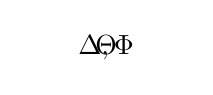
\begin{tikzpicture}[
				sibling distance=30pt, level distance=60pt, 
				t/.style={text height=1.5ex, text depth=.25ex, rectangle, outer sep=0pt}]
			\Tree
				[
					\edge[unary] node[left, midway] {\dep{d}};	
						[\edge[roof, dashed]; \node[t] {\hphantom{123}$\Delta,\Phi$\hphantom{123}};]
					\edge[unary] node[yshift={-7pt}, xshift={11pt}] {\dep{x}}; \node[t,xshift=0pt] {$\Theta$};
				]
			\end{tikzpicture}
			&
			\raisebox{60pt}{$\xleftarrow{\Extraction}$}
			&
			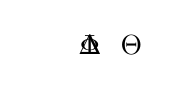
\begin{tikzpicture}[
				sibling distance=7.5pt, level distance=40pt, 
				t/.style={text height=1.5ex, text depth=.25ex, rectangle, outer sep=0pt}, node distance=10pt]
			\tikzset{level 1/.style={level distance=33pt}}
			\tikzset{level 2/.style={level distance=47pt}}
			\tikzset{frontier/.style={distance from root=120pt}}
			\Tree
				[
					\edge node[midway, right] {\dep{d}}; 
					[
						[
							\edge[roof, dashed]; \node[t] {\hphantom{123}$\Delta$\hphantom{123}};
						]
						\edge[unary] node[midway, right] {\dep{x}}; \node[t, xshift={15pt}] {$\Theta$};
						[
							\edge[roof, dashed]; \node[t] {\hphantom{123}$\Phi$\hphantom{123}};
						]
					]
				]
			\end{tikzpicture}
		\end{tabularx}
		\caption{Corresponding tree transformation.}
		\label{subfigure:extraction_tree}
	\end{subfigure}
	\caption{Controlled extraction in the dependency-bracketed setting.}
	\label{figure:modal_dep_extraction}
\end{figure}

Naively, we would assume that the absence of binary bracketing structure in $\LC$ would allow us direct access to the gap within the relative clause body, counteracting the need for the control modalities of (\ref{equation:objrel}).
But the gap is still enclosed, except this time under layers of impenetrable dependency domains!
Seems like we need to reinstate control -- both kinds of modalities must be employed in tandem;
although in truth, the two do not really constitute distinct kinds \textit{per se}: they only differ insofar as their linguistic purposes do.
Nevertheless, it might be handy to make a notational distinction between them, just for the sake of reading comprehension.
From now on, we will use filled symbols to denote control modalities (i.e. ones whose purposes are confined to rebracketing and movement), and white symbols to denote dependency modalities (i.e. ones whose purpose is linguistic annotation, and the brackets of which we expect to see in the antecedent of the proof's end yield).
Even when having a single control pair, assigning it an explicit label \dep{x} is still useful, since it will allow us to tell its brackets apart from the rest.
In this regime, our relativizer's type assignment becomes:
\begin{equation}
\text{that} :: \subcat{l}{rel}{o} := \dbox{mod}(\np\divleft\np)\divright\ddia{body}(\s\divright\dxdia{x}\dxbox{x}\ddia{obj}\np)
\end{equation}
which is faithful to both (\ref{equation:deprel}) and (\ref{equation:objrel}), as it conveys that the missing object is now \textit{movable}.


\begin{figure}
	\smaller[2]
	\[
		\infer[\divright E]{\w{that}, \dbra{\dbra{\dbra{\w{the}}{det}, \w{eye}}{su}, \w{may}, \dbra{\dbra{\w{never}}{mod}, \w{behold}}{vc}}{body} \vdash \dbox{mod}(\np\divleft\np)}{
			\infer[\Lex]{\w{that} :  \subcat{l}{rel}{o}}{}
			&
			\hspace{-50pt}
			\infer[\ddia{body}I]{\dbra{\dbra{\dbra{\w{the}}{det}, \w{eye}}{su}, \w{may}, \dbra{\dbra{\w{never}}{mod}, \w{behold}}{vc}}{body} \vdash \ddia{body}(\s\divright\ddia{obj}\np)}{
				\infer[\divright I]{\dbra{\dbra{\w{the}}{det}, \w{eye}}{su}, \w{may}, \dbra{\dbra{\w{never}}{mod}, \w{behold}}{vc} \vdash \s\divright\ddia{obj}\np}{
					\infer[\dxdia{x}E]{\dbra{\dbra{\w{the}}{det}, \w{eye}}{su}, \w{may}, \dbra{\dbra{\w{never}}{mod}, \w{behold}}{vc}, \varj \vdash \s}{
						\infer[\divleft E]{\dbra{\dbra{\w{the}}{det}, \w{eye}}{su}, \w{may}, \dbra{\dbra{\w{never}}{mod}, \w{behold}}{vc}, \dbra{\vari}{x} \vdash \s}{
							\infer*{\dbra{\dbra{\w{the}}{det}, \w{eye}}{su} \vdash \ddia{su}\np}{	}
							&
							\infer[\divright E]{\w{may}, \dbra{\dbra{\w{never}}{mod}, \w{behold}}{vc}, \dbra{\vari}{x} \vdash \gtype{itv}}{
								\infer[\Lex]{\w{may} : \gtype{aux}}{}
								&
								\hspace{-25pt}\infer[\Extraction]{\dbra{\dbra{\w{never}}{mod}, \w{behold}}{vc}, \dbra{\vari}{x} \vdash \ddia{vc}\gtype{itv}}{
									\infer[\ddia{vc}I]{\dbra{\dbra{\w{never}}{mod}, \w{behold}, \dbra{\vari}{x}}{vc} \vdash \ddia{vc}\gtype{itv}}{
										\infer[\divright E]{\dbra{\w{never}}{mod}, \dbra{\vari}{x} \vdash \gtype{itv}}{
											\infer[\dbox{mod}E]{\dbra{\w{never}}{mod} \vdash \gtype{itv}\divright\gtype{itv}}{
												\infer[\Lex]{\w{never} : \gtype[l]{adv}_{\divright}}{}
											}
											&
											\infer[\divright E]{\w{behold}, \dbra{\vari}{x} \vdash \gtype{itv}}{
												\infer[\Lex]{\w{behold}: \gtype[l]{tv}}{}
												&
												\infer[\dxbox{x} E]{\dbra{\vari}{x} \vdash \ddia{obj} \np}{
													\infer[\Ax]{\vari : \dxbox{x}\ddia{obj}\np}{}
												}
											}
										}
									}
								}
							}
						}
						&
						\hspace{-60pt}
						\infer[\Ax]{\varj : \dxdia{x}\dxbox{x}\ddia{obj}\np}{}
					}
				}
			}
		}
	\]
	\caption{Dependency-enhanced adaptation of the proof of Figure~\ref{subfigure:lovecraft_rel_clause:rc}, exemplifying the interaction between dependency and control modalities.}
	\label{figure:lovecraft_dep_rep_clause}
\end{figure}


Mobility, however, also means something different now.
Taking inspiration from the established structural vocabulary (see Figure~\ref{figure:modal_structural_rules} if you need to jog your memory), we need to concoct a novel structural rule: one that allows the \textit{extraction} of a nested substructure under the appropriate bracketing conditions.
The magical conconction is presented in Figure~\ref{subfigure:extraction_rule}.
Within arbitrary context $\Gamma$, it looks for a \dep{d}-labelled unary tree enclosing a \dep{x}-labelled unary tree $\Theta$ wrapped by sequences $\Delta$ to the left and $\Phi$ to the right.
There, it allows us to pull the $\Delta$ out, casting the outermost unary tree into a binary sequence and assigning \dep{d} to the concatenation of $\Delta$ and $\Phi$ alone. 
If this makes little sense, see Figure~\ref{subfigure:extraction_tree} for a visual rendition.
If still unclear, move your mental cursor four sentences back (this one included) and try again.

Equipped with this missing bit of alchemical understanding, we're at long last able to produce analyses for some less contrived linguistic examples; Figure~\ref{figure:lovecraft_dep_rep_clause} presents the dependency-enhanced derivation we set out to deliver.
Before we move on, though, some important observations are in order.
First, the presentation makes an implicit quantification over the outer label, \dep{d} -- if we were to be really pedantic, we'd need a unique instantiation of that rule for each dependency (but not control!) modal label in the logic.
Beyond a bookkeeping obligation, this parameterization can also be to our advantage: it allows us to directly control which of the dependency domains allow extraction, and which do not.
On a less bureaucratic note, the contextual formulation of the rule carries the usual problem of complicating syntactic equality checking. 
In practice, we can employ a localized version, i.e. one where $\Gamma$ is a flat context (i.e. a sequence with a hole), which means that extractions need to be preemptively applied before every bracketing operation, rather than deferred and done in bulk in the future.
Finally, it is important to remember that the rule is supplementary to (and \textit{not} a substitute for) controlled associacitivity and/or commutativity: altering the linear order of substructures in $\LC$, or their binary brackets in $\NL$, still calls for different structural rules with possibly different control modalities that will need to coexist with the \Extraction{} rule for structures to find their intended positions.


\paragraph{Ever higher order}
The example just inspected hides a crucial wisdom: variable abstraction applies to variables -- \textit{not} complex structures thereof.
Control modalities may impose transient bracketing structure upon hypotheses, temporarily hindering their abstraction, but it is always retroactively redacted with the $\diamond E$ rule (after all the necessary structural operations have taken effect).
The bracketing imposed by dependency modalities, however, is built to last, posing a potential roadblock to hypothetical reasoning and higher-order types.

Hypothetical complements are relatively easy to tackle: they just come packed with their diamonds at variable instantiation time.
Excluding the presence of the irrelevant control box, this is exactly the strategy followed in the example under scrutiny (see the $\Ax$ rule intantating $\vari$ in Figure~\ref{figure:lovecraft_dep_rep_clause}).
Upon closer inspection, we can verify that this is in fact just the $\eta$ normalized version of hypothesizing a plain type, assigning it the desired dependency brackets via the $\diamond I$ rule, and then performing a substitution of the bracketed variable for a logical equivalent (wrapped under the necessary control brackets) via the $\diamond E$ rule -- consult Figure~\ref{figure:eta_normalized_complement_hypothesis} and contrast with Figure~\ref{subfigure:modal_eta_reductions} if unconvinced.

\begin{figure}
	\begin{tabularx}{0.9\textwidth}{@{}cCc@{}}
	$
		\infer[\ddia{obj} E]{\dbra{\vari}{x} \vdash \ddia{obj}\np}{
			\infer[\ddia{obj} I]{\dbra{\vark}{obj} \vdash \ddia{obj}\np}{
				\infer[\Ax]{\vark : \np}{}
			}
			&
			\infer[\dxbox{x} E]{\dbra{\vari}{x} \vdash \ddia{obj}\np}{
				\infer[\Ax]{\vari : \dxbox{x}\ddia{obj}\np}{}
			}
		}
	$
	&
	\raisebox{10pt}{$\overset{\eta}{\equiv}$}
	&
	$
		\infer[\dxbox{x} E]{\dbra{\vari}{x} \vdash \ddia{obj} \np}{\infer[\Ax]{\vari : \dxbox{x}\ddia{obj}\np}{}}
	$
	\end{tabularx}
	\caption{$\eta$ long form of the $\ddia{obj}$ connective of hypothesis $\vari$  in Figure~\ref{figure:lovecraft_dep_rep_clause}.}
	\label{figure:eta_normalized_complement_hypothesis}
\end{figure}

Hypothetical adjuncts are less forgiving.
A hypothesized adjunct will seek to apply itself to some phrasal head, which is impossible unless it first drops its box.
But in dropping its box, it becomes enclosed in structural dependency brackets that prohibit its eventual abstraction.
We will need to once more resort to the $\diamond E$ rule to remove , except this time it will be the interior combination of Figure~\ref{subfigure:modal_properties:interior} that we are invoking, not subject to $\eta$ contraction.
To see this in action, let us once more consider an excerpt from our go-to source: \textex{a city of high walls where sterile twilight reigned}%
\footnote{H.P. Lovecraft, \textit{Azathoth} (1938). In \textit{Leaves} (2).}.
The relative adverb \textex{where} heads yet another a relative clause, \textex{where sterile twilight reigned}, acting as a postnominal modifier to the noun phrase \textex{a city of high walls}.
The relative clause differs to the ones so far inspected, in missing from its embedded subordinate \textex{sterile twilight reigned \gap} not a complement, but an adjunct: a gap-equivalent to the lexical \textex{there} of Figure~\ref{subfigure:opiate_oceans_poured_there}, except dependency-enhanced, i.e. $\dbox{mod}(\smallgtype{itv}\divleft\smallgtype{itv})$ in shorthand.
As Figure~\ref{subfigure:higher_order_dep:erasure} illustrates, the need for bracket erasure necessitates prefixing the gap type with a residual diamond, steering us towards our first ever fourth order type:
\begin{equation}
\text{where} :: \subcat{l}{rel}{loc} := \dbox{mod}(\np\divleft\np)\divright\ddia{body}(\s\divright(\ddia{mod}\dbox{mod}(\smallgtype{itv}\divleft\smallgtype{itv}))
\end{equation} 
This beast of a type plays the starring role in the derivation of Figure~\ref{figure:higher_order_dep}; it promises to provide a postnominal modifier, if presented with a (third order) relative clause body, that being a sentence missing to its right a diamond-marked (second order) postverbal modifier.

\begin{figure}
	\begin{subfigure}{1\textwidth}
		\smaller
		\[
			\infer[\divleft E]{\w{reigned}, \varj \vdash \gtype{itv}}{
				\infer[\Lex]{\w{reigned} : \gtype{itv}}{}
				&
				\infer[\ddia{mod}E]{\varj \vdash \gtype{itv}\divleft\gtype{itv}}{
					\infer[\dbox{mod}E]{\dbra{\vari}{mod} \vdash \gtype{itv}\divleft\gtype{itv}}{
						\infer[\Ax]{\vari : \dbox{mod}(\gtype{itv}\divleft\gtype{itv})}{}
					}
					&
					\infer[\Ax]{\varj : \ddia{mod}\dbox{mod}(\gtype{itv}\divleft\gtype{itv})}{}
				}
			}
		\]
		\caption{Structurally freeing a hypothesized adjunct...}	
		\label{subfigure:higher_order_dep:erasure}
	\end{subfigure}\\[\midsep]
	\begin{subfigure}{1\textwidth}
		\smaller
		\[
			\infer[\!\divright E]{\w{where}, \dbra{\dbra{\dbra{\w{sterile}}{mod}, \w{twilight}}{su}, \w{reigned}}{body} \vdash \dbox{mod}(\np\divleft\np)}{
 				\infer[\!\!\Lex]{\w{where} : \subcat{l}{rel}{loc}}{}
				&
				\hspace{-5pt}
				\infer[\!\!\ddia{body}I]{\dbra{\dbra{\dbra{\w{sterile}}{mod}, \w{twilight}}{su}, \w{reigned}}{body} \vdash \ddia{body}(\s\divright(\ddia{mod}\dbox{mod}(\gtype{itv}\divleft\gtype{itv})))}{
					\infer[\divright I]{\dbra{\dbra{\w{sterile}}{mod}, \w{twilight}}{su}, \w{reigned} \vdash \s\divright(\ddia{mod}\dbox{mod}(\gtype{itv}\divleft\gtype{itv}))}{
						\infer[\divleft E]{\dbra{\dbra{\w{sterile}}{mod}, \w{twilight}}{su}, \w{reigned}, \varj \vdash \s}{
							\infer[\ddia{su}I]{\dbra{\dbra{\w{sterile}}{mod}, \w{twilight}}{su} \vdash \ddia{su}\np}{
								\infer[\divright E]{\dbra{\w{sterile}}{mod}, \w{twilight} \vdash \np}{
									\infer[\dbox{mod}E]{\dbra{\w{sterile}}{mod} \vdash \np\divright\np}{
										\infer[\Lex]{\w{sterile} : \gtype{adj}_{\divright}}{}
									}
									&
									\infer[\Lex]{\w{twilight}: \np}{}
								}
							}
							&
							\infer{\w{reigned}, \varj \vdash \gtype{itv}}{\text{(\ref{subfigure:higher_order_dep:erasure})}}
						}
					}
				}
			}
		\]
		\caption{...to provide a gap in the higher-order argument of the relative adverb \textex{where}.}
		\label{subfigure:higher_order_dep:rc}
	\end{subfigure}
	\caption{Deriving a locative relative clause.}
	\label{figure:higher_order_dep}
\end{figure}

But why go through all this trouble of producing the dependency brackets only to then immediately cancel them out?
The alternative of hypothesizing a plain functor without any dependency markings would be logically valid but grammatically suboptimal and contrary to our agenda, as it would give us no insights on what the dependency function of the gap is; the modalities stay.
Another, more pressing question is that of the compatibility between hypothetical adjuncts and the control modality of the previous paragraph, i.e. how could we deal with the nested gap in e.g. \textex{where sterile twilight \textbf{may} reign \gap}.
Fortunately, we need not worry: our previous treatment still holds with only the most minor of adjustments.
Same as before, we have to alter the typing of the gap by prepending a boundary crossing permit, the interior pair $\dxdia{x}\dxbox{x}$.
As the modal chains are no longer $\eta$ contractable, the gap will manifest as three distinct variables, sequentially substituting one for another via two $\diamond E$ rules, as shown in Figure~\ref{figure:higher_order_nested_dep}.
The first substitution of $\vari$ for $\varj$ is responsible for removing the \dep{mod} brackets for \dep{x} ones, allowing any applications of the \Extraction{} rule in the telescoped subproof $s$.
The bracketed variable will eventually be positioned at the outermost branch of the antecedent tree, at which point it can be substituted for $\vark$, the ``true'' variable of the gap.
Don't give in to despair; this is peak complexity -- with these type patterns at our disposal we should be able to tackle any linguistic phenomenon we might encounter from this point on.
Note, finally, that complement and adjunct gaps are not that different to one another after all: they both mimic their corresponding lexical assignment (a plain type or a boxed functor, respectively), except prepended by a diamond of whichever dependency role they will assume and (if needed) a structural extraction licensor.


\begin{figure}
	\smaller
	\[
		\infer{\vdots}{
			\infer[\dxdia{x} E]{\dbra{\Gamma}{d}, \vark \vdash \prop{A}}{
				\infer*[s]{\dbra{\Gamma}{d}, \dbra{\varj}{x} \vdash \prop{A}}{
					\infer[\ddia{mod} E]{\dbra{\varj}{x} \vdash \gtype{itv}\divleft\gtype{itv}}{
						\infer[\dbox{mod} E]{\dbra{\vari}{mod} \vdash \gtype{itv}\divleft\gtype{itv}}{
							\infer[\Ax]{\vari : \dbox{mod}(\gtype{itv}\divleft\gtype{itv})}{}
						}
						&
						\infer[\dxbox{x} E]{\dbra{\varj}{x} \vdash \ddia{mod}\dbox{mod}(\gtype{itv}\divleft\gtype{itv})}{
							\infer[\Ax]{\varj : \dxbox{x}\ddia{mod}\dbox{mod}(\gtype{itv}\divleft\gtype{itv})}{}
						}
					}
				}
				&
				\hspace{-40pt}
				\infer[\Ax]{\vark : \dxdia{x}\dxbox{x}\ddia{mod}\dbox{mod}(\gtype{itv}\divleft\gtype{itv})}{}
			}
		}
	\]
	\caption{Schematic pattern for extracting a nested hypothetical adjunct.}
	\label{figure:higher_order_nested_dep}
\end{figure}

\subsection{Interfaces}
Having completed our tour of dependency-decorated proofs, it is time for respite and reflection.
Let us take a moment to internalize where we started from and where we are now.

\subsubsection{Dependency Trees}
Our first ambition was to provide categorial type logics with the means necessary to argue about dependency relations, ideally subsuming dependency trees within the logic's antecedent structures. 
To claim our endeavour a success, we need to actually \textit{show} how these dependency trees can be extracted.

Let's begin with some trivial observations.
In the domain of dependency annotated proofs, endsequents will contain neither variables nor any control brackets.
Collapsing any notion of structure imposed by the functional core (i.e. drop constituency and word order from the builtin structural binder, since dependency trees are agnostic to those), we end up with structures made exclusively of constants (terminal nodes), multisets of structures (unordered variadic branches) and dependency enclosed structures (unary branches).
This typological description can be further refined by noticing that the non-zeroary tree operators alternate in turns: there's no chaining of unary brackets (each phrase is only assigned at most one dependency role), nor a multiset of multisets (as the simplified structural binder is flat).
Finally, consider that each multiset will coincide with a dependency domain, containing exactly one (unmarked) head constant (necessarily a word), some $n$ adjuncts and some $m$ complements.

With these in mind, we arrive at the following (modulo permutation) inductive definition of a dependency induced structure:
\begin{equation}
	\Gamma
		 	:=  
 	\underbrace{\dbra{\Gamma_0}{d_0} \dots \dbra{\Gamma_{n-1}}{d_{n-1}}}_{\text{adjuncts}} \ 
	\underbrace{\dbra{\Gamma_n}{d_n} \dots \dbra{\Gamma_{n + m - 1}}{d_{n + m -1}}}_{\text{complements}} \ 
	\underbrace{\vphantom{\Gamma_0^a}\kappa}_{\text{head}} \
\end{equation}
Converting such a structure to a dependency tree akin to the one of Figure~\ref{figure:udparse} is pleasantly easy: just apply the function below to it (plug an invisible ``root'' node and label to get things going).%
\footnote{For the more verbally inclined, we need to simply enter every dependency domain and establish an arc from the local head to (the head of) each of its dependents.}
\begin{align*}
& \mathsf{deptree :: Struct \to Head \to \deps \to Set[Arc]}\\
& \mathsf{deptree} \ 
			\left(\dbra{\Gamma_0}{d_0} \dots \dbra{\Gamma_{n + m - 1}}{d_{n + m -1}} \ 
			\kappa\right)
			\ 
			\mathsf{root}
			\ 
			\mathsf{label} = \\
& \quad	
			 \{ \mathsf{root} \xrightarrow{\mathsf{label}} \kappa \}
			\cup \raisebox{0pt}[0pt]{$\bigcup\limits_{i=0}^{n+m-1}$}\{\mathsf{deptree} \ \Gamma_i \ \ \kappa \ \ d_i\}
\end{align*}
Figure~\ref{figure:example_deps} shows the function's yield applied to two of the section's example derivations.
Given a partition of $\deps$ into adjuncts and complements, the conversion can trivially be extended with the bidirectional dependency arcs described in Section~\ref{subsection:dep_grammars}.
Word order is also straightforward to capture, if we just keep the structural order provided by a non-commutative calculus intact.
In any case, our efforts go to show that the general structure of a dependency tree can easily be captured by a dependency-enhanced type logic using the type assignment patterns discussed.
Aligning the type logic to a specific flavour of a dependency grammar was never our main intention, but should be fairly easy to accomplish by reverse-engineering the annotational specifics of the target: a task for future generations.

\begin{figure}
	\centering
	\begin{subfigure}{1\textwidth}
		\centering
		\begin{tikzpicture}[t/.style={text height=1.5ex, text depth=.25ex, rectangle, outer sep=0pt}, node distance=10pt]
		\smaller
		\node[t] (that)		at (0,0) {\w{that}};
		\node[t] (the)		[right=10pt of that] {\w{the}};
		\node[t] (eye)		[right=10pt of the] {\w{eye}};
		\node[t] (may)		[right=10pt of eye] {\w{may}};
		\node[t] (never)	[right=10pt of may] {\w{never}};
		\node[t] (behold)	[right=10pt of never] {\w{behold}};
		\path[->] (that) [bend left=75] edge node [above] {\smaller[2]{body}} (may);
		\path[->] (may) [bend right=50] edge node [above] {\smaller[2]{su}} (eye);
		\path[->] (eye) [bend right=50] edge node [above] {\smaller[2]{det}} (the);
		\path[->] (may) [bend left=70] edge node [above] {\smaller[2]{vc}} (behold);
		\path[->] (behold) [bend right=40] edge node [above] {\smaller[2]{mod}} (never);
		\end{tikzpicture}
		\caption{Dependency tree of $\ctx{\w{that}, \dbra{\dbra{\dbra{\w{the}}{det}, \w{eye}}{su}, \w{may}, \dbra{\dbra{\w{never}}{mod}, \w{behold}}{vc}}{body}}$.}
		\label{subfigure:that_the_eye_may_never_behold_deps}
	\end{subfigure}\\[\midsep]
	\begin{subfigure}{1\textwidth}
	\centering
		\begin{tikzpicture}[t/.style={text height=1.5ex, text depth=.25ex, rectangle, outer sep=0pt}, node distance=10pt]
		\smaller
		\node[t] (where)		at (0,0) {\w{where}};
		\node[t] (sterile)		[right=10pt of where] {\w{sterile}};
		\node[t] (twilight)		[right=10pt of sterile] {\w{twilight}};
		\node[t] (reigned)		[right=10pt of twilight] {\w{reigned}};
		\path[->] (where) [bend left=55] edge node [above] {\smaller[2]{body}} (reigned);
		\path[->] (reigned) [bend right=40] edge node [above] {\smaller[2]{su}} (twilight);
		\path[->] (twilight) [bend right=40] edge node [above] {\smaller[2]{mod}} (sterile);
		\end{tikzpicture}
		\caption{Dependency tree of $\ctx{\w{where}, \dbra{\dbra{\dbra{\w{sterile}}{mod}, \w{twilight}}{su}, \w{reigned}}{body}}$.}
		\label{subfigure:where_sterile_twilight_reigned_deps}
	\end{subfigure}
	\caption{Trees extracted from the derivations of Figures~\ref{figure:lovecraft_dep_rep_clause} (\subref{subfigure:that_the_eye_may_never_behold_deps}) and~\ref{figure:higher_order_dep} (\subref{subfigure:where_sterile_twilight_reigned_deps}).}
	\label{figure:example_deps}
\end{figure}

\subsubsection{Semantics}
The trees of Figure~\ref{figure:example_deps} leave something to be desired: by backpedaling towards dependency grammars, higher-order phenomena have been completely dismissed -- wasted are all our efforts to tame and manage the bracketing structures of hypotheses.
Perhaps importing residuated modalities just for the sake of cracking some dull and flat dependency relations was an overkill after all?
The answer is no.
Antecedent bracketing structures is but the most superficial aspect of our grammar logic's proofs -- the function argument relations of the implicational core are retained, and in fact coexist with the dependency annotations (including higher-order ones) in the logic's term calculus, which we have been unjustly ignoring.

The far richer type and term structure of the syntactic calculus creates, in turn, ample opportunity for the passage to semantics.
We are of course still presented with the cautious option of simply forgetting about dependencies, retracting to the same dependency agnostic $\ILL$ we did earlier.
But the radical path would have us preserve dependency operators in the intermediate station of derivational semantics%
	\footnote{And thus necessarily also the extraction pair $\dxdia{x}$, $\dxbox{x}$.},
in hope of them findind downstream applications later on.
A first merit would be the availability of richer type assignments in the lexical semantics domain, where previously identical function types become distinguishable by virtue of their modal decorations.
There, syntactic modalities can be translated to semantic operators, lifting the target signature accordingly -- \textit{monads} make for a natural choice~\cite{kobayashi1997monad}.
Furthermore, dependents are delineated and identified by their syntactic roles, allowing distinct semantic treatments, if so desired.
Even in the modest setting of a non-inflated translation, modalities can help tell which of the (possibly many) combinations of semantic slots are occupied in a given construction, allowing the correct compositional recipe to be retrieved from the semantic lexicon.
In the edge case, they open the possibility for a homomorphic translation that ``forgets'' parts of the implicational directives of the logic, relying instead on the source dependency markings for the construction of its semantic terms.


\section{Key References \& Further Reading}
\label{section:references_2}
The chapter has presented novel work, assembled and expanded from streamlined bits and pieces of earlier published drafts.
The good news is you're reading the most extensive overview available at the time of writing.
The bad news is I don't have much references for you -- if it's any consolation, there's still two more chapters to go.
Of work not included in this chapter or the ones to come, the one by \citet{rouss} has dependency modalities play a key role in the annotation and generation of complex verb clusters with subtle semantic dependencies, the recursive nature of which seems to break the omnipotence attributed to neural language models.
For a less avant-garde reading, I'd like to draw your attention to this chapter's historical roots, namely the manuscript of \citet{moortgat1991heads}.
If unsated you crave for more modalities-as-dependencies, you have the option of either writing something yourself or waiting until someone else does.\footnote{Calling it now, next big development in Moortgat et al. [2051].}

More broadly and outside their use as dependency markers, unary modalities have long now been a tempting way to encode linguistic features -- see \citet{moa} and \citet{10.7551/mitpress/6169.003.0012,johnson1999resource}, for instance.
Further away from our niche territories, the relation between dependency grammars and lexicalism is extensively analyzed by \citet{kuhlmann2010dependency}, who asks (and answers) the question of which formal grammars induce what kind of dependency structures.
On a relevant note, the slightly disheveled categorial dependency grammars make for an attempt to provide a categorial treatment of dependency structure, where the arcs and their labels are themselves the grammar's propositional constants~\cite{dekhtyar2015categorial}.
For even more general literature on constituency grammars, dependency grammars or instantiations thereof, I will unfortunately have to direct you towards your favorite web search engine.

\bibliographystyle{abbrvnat}
\bibliography{bibliography}